\section{Methods}
The first part of this chapter provides an overview of the related work in the field of
thematic cartography. This topic is going to be combined with basic principles of visualizations and visual design principles. Afterwards, \ac{GeoVis} is explained from a practical point of view and the connections to close related fields are made. This rather high level discussion is followed by a more specialized view on four different map-based visualizations. The combination of thematic cartography and interaction leads to the next sections, where different interaction approaches are explained in detail. Finally the current state in the domain of map-based visualization tools is analysed, summarized and potential improvements are identified.

\subsection{Thematic Cartography}
\label{s:cartography}
\cbstart
This Chapter discusses the concept used for animated transitions between geo-spatial visualisations, as well as the evaluation and implementation of the concept.
The first Section of this Chapter deals with the concept of this thesis and its limitations. An abstract analysis with the framework provided by \citeauthor{Munzner2014} is made. The findings of the conducted user study their limitations created by the study design are also part of the first Section. The second part presents strengths and weaknesses of the implemented application. Therefore, each Section provides answers of the derived research question.
\cbend

\subsection{Conceptual Discussion and Conceptual Limitations}
% marc fragen, was hier noch stehen soll
% \subsubsection{Analysis-Framework}
The implemented web application is based on two datasets: a tabular dataset (SuperStore-Sale) and a geo-spatial one (boundaries). These datasets are statically preprocessed and used. This information already answers the question of what the application visualises.

\cbstart
Furthermore, the main objective of the visualisations is to consume information, according to Figure \ref{fig:why} on page \pageref{fig:why}. In addition, users of the application should discover previously unkown knowledge. Considering the performed user study and its task, a user should discover an area in the United States which has the most orders normalized by population.
\cbend

Overall, the application uses static encodings like colour, size and shapes for the different types of maps and motion when changing the visual appearance. This already leads to the possibilities in manipulation. Changing the level of detail, colour scheme and particle speed allow for exploring different settings. However, reducing or changing the displayed information is not possible at all. The implemented types of maps have very specific characteristics, making a consistent aggregation or filtering of information impracticable.


\newpage
\subsection{Technical Discussion and Technical Limitations}
The web application consists of two main parts: the first one is the data acquisition and preparation and the second one is the transition manager handling the animation. The first subsection will discuss the restrictions, advantages and disadvantages coming along with the implementation. This discussion is followed by pointing out the strengths and weaknesses of using the transition manager. The discussion is concluded with an analysis of the used technology.

\subsubsection{Data Acquisition and Data Preparation}
Automatic data acquisition and preparation with GNU-Make is very powerful and flexible. The primal strength of it is that writing a \textit{Makefile} creates a machine-readable documentation for the whole workflow. Recording each step in the process enables reproducibility later on.
Thinking of GNU-Make as a dependency graph is key. Unlike a linear and sequential script, a dependency graph is more modular. For example, a \textit{Makefile} is augmentable with deriving multiple data files from the same zip archive without repeating the download of the archive. Thus, using GNU-Make fulfills already two requirements: it scales very well if using multiple data files from different data sources is desired and modularity is provided with the ability of defining tasks for different concerns. However, one major weakness of GNU-Make is its syntax and possible complexity. Putting the facts into comparison, the advantages outweigh the disadvantages.

The primary setup of pre-calculating every needed information has one major advantage as well as one disadvantage. The client-side web application needs to deliver the file to the client with all information only once. Afterwards, everything can be used without dynamically calculating values. On the one side, the initial loading time of the application is significantly higher compared to only delivering the boundary informations. On the other hand, the acquisition and calculation of data later yields to performance drops whenever the data is needed.
A significant drawback using this setup is that showing additional information to an aggregated symbol is not possible. A thematic map based on aggregation fully relys on the preprocessed dataset. Therefore, showing additional information on the dot-map would make use of the Superstore-Sale dataset with all information accessible, whereas showing additional information for symbols or units in aggregated thematic maps depends on the preprocessed boundary file. From an abstract point of view, the practical implementation uses two different source files for showing one phenomenon, yielding to inconsistency when allowing interaction with the visualisation. Changing the visual appearance also changes their base-data and therefore consistency in interaction concepts is not possible and therefore left out.

\subsubsection{Transition Manager}
The implemented transition manager is a key part of the practical application. It specifies some kind of structure to all visualisation classes. Each step of a transition needs to be implemented in the actual class and the manager only calls the exposed functions in the correct order to create the animated transition. This concept ensures separation of concerns of each exposed function and therefore guaranteeing modularity in creating animated transitions.

The transition table \ref{tab:transition-table} on page \pageref{tab:transition-table} mentions shape transitions which are not yet implemented. This is due to the GeoJSON file acquired from the census bureau. Every enumeration unit is specified as a multipolygon. The GeoJSON specification defines multipolygons as a collection of polygons and polygons as an array of coordinates. However, a polygon can contain multiple rings. If this is the case, the first ring must be the exterior one and any others must be interior rings or holes.
Animating the morphing of an enumeration unit to a symbol would require the starting point to be a polygon in order to create a smooth transition. However, merging the multipolygon of an enumeration unit to a single polygon containing only a single outer ring is not possible. A point in the multipolygon and therefore in the map is unique. This makes it impossible to find the outer ring of multiple polygons.
Another possibility in animated morphing would be to morph each polygon to a particular segment of the symbol. With the current data, the transition will not look smooth. Some polygons in enumeration units are hidden behind the default symbol, therefore an animated morphing of those would look like a random symbol segment appearing without noticing the origin of the polygon.


\subsubsection{Used Technology}
Using ECMAScript6 was not the best choice. Decker presents ECMAScript6 polyfill performance tests. He implements a specific feature with multiple JavaScript versions and compairs their runtime. Furthermore, he uses multiple different transpilers yielding considerable results. The following discussion only includes features which are used in the practical application. It also focuses on the results for Chrome 51, because this is the browser version used for testing the application \iacite{Decker2016}.

His report\footnote{See \href{https://kpdecker.github.io/six-speed/}{https://kpdecker.github.io/six-speed/} for more information.} shows that using classes in combination with babel as a transpiler is $1,8\times$ slower in chrome 51 compared to the default way of creating an object in JavaScript. In addition, using default parameters and calling a parent class with the super keyword is significantly slower. However, the usage of promises is a little bit faster in Chrome 51 \iacite{Decker2016}.

Nonetheless, comparing the used version of JavaScript with its performance with its readability, it is still reasonable because of the better maintainability of the code. Despite its advantage, it is still needed to consider using a different transpiler or JavaScript version if the application should use larger datasets or lacks performance.

\ac{D3} is a proper library providing a huge set of useful functions. Its flexibility and functional style allows code reuse. The usage of this library in the practical application shows no drawbacks at all. Animating all symbols at once or with different timings and applying forces such as gravity is neither a performance problem, nor an implementation problem. However, using \ac{DOM} elements always depends on a proper use of JavaScript. For example, considering a memory leak because of keeping references to deleted \ac{DOM} elements would result in an unresponsive browser.

\ac{Pixi} does not show any disadvantage in the currently implemented application. Displaying particles as sprites is a very scaleable way and animating them with a generalised render function combined with an animation queue provides modularity.


\subsubsection{Geographic Visualization}

\subsubsubsection{Dot}

\subsubsubsection{Proportional Symbol}

\subsubsubsection{Choropleth}

\subsubsubsection{Cartogram}

\subsection{Interaction in visualizations}
\label{s:interaction}

\subsubsection{Overview First, Focus + Zoom}

\subsubsection{Zoom and Filter}

\subsubsection{Details on Demand}

\subsubsection{Multiple Views, Linking \& Brushing}

\subsubsection{Transitions}

\subsection{State-of-the-art application analysis}


% \subsection{Geovisualization}
% In modern geovisualization software, such data are represented using both traditional cartographic techniques based on the use of colours, textures, symbols, and diagrams; and using computer-enabled techniques such as map animation and interactive 3D views. Moreover, maps are used in combination with nongeographic visualization techniques such as scatterplots or parallel coordinates. The use of multiple interactively linked views providing different perspectives into the data has become a kind of standard in geovisualization. However, a number of problems have yet to be solved, such as the scalability of geovisualization tools and their usability.

% GEO VIS
% Thus visualization now also emphasizes the knowledge creation and hypothesis generation aspects of \ac{SciVis}.

% As already mentioned, \ac{GeoVis} is closely related to the fields of \ac{SciVis} and also \ac{InfoVis} and emphasizes knowledge construction over knowledge storage or information transmission \iacite{maceachren:1997}. However \ac{InfoVis} needs to be strictly differentiated from \ac{SciVis}. \ac{InfoVis} deals with abstract data like for example movies in a movie database whereas \ac{SciVis} operates on real-world data with spatial character.

% \ac{GeoVis} also contributes significantly to other related fields such as \ac{SciVis} and also \ac{InfoVis}. Owing to its roots in cartography, \ac{GeoVis} contributes to these other fields by way of the map metaphor, which "[\ldots] has been widely used to visualize non-geographic information in the domains of information visualization and domain knowledge visualization" \iacite{Jiang2005}. It emphasizes knowledge construction over knowledge storage or information transmission \iacite{maceachren:1997}. However \ac{InfoVis} needs to be strictly differentiated from \ac{SciVis}. \ac{InfoVis} deals with abstract data like for example movies in a movie database whereas \ac{SciVis} operates on real-world data with spatial character.

% Traditional, static maps have a limited exploratory capability. The graphical representations are inextricably linked to the geographical information beneath. \ac{GIS} and \ac{GeoVis} allow for more interactive maps. Both of them have the ability to extend the basic layer of a map with user-experience abilities like for example zooming in or out and to change the visual appearance of the map \iacite{Jiang2003}.

% This kind of visualization is also used in practical applications. The following list shows some summarized examples of those:
% \begin{description}

% \item[Urban Planning] \hfill \\
% Urbanists use \ac{GeoVis} to "[\ldots] model environmental interests and policy concerns of the general public" \iacite{Jiang2003}. \citeauthor{Jiang2003} also mention two examples, in which "[\ldots] 3D photorealistic representations are used to show urban redevelopment and dynamic computer simulations are used to show possible pollution diffusion over the next few years".

% \citeauthor{Jiang2003} also describe that the widespread use of the internet by the general public allows collaborative planning to be conducted in both centralised and decentralised manner. The former way of planning in committee rooms or computer facility rooms can be extended with a decentralised web platform. This platform would lead to increased parcitipation by the public because
% \begin{enumerate}
% \item the internet already integrates various interactive and proactive techniques and
% \item is time and place independent.
% \end{enumerate}

% \item[Environmental Studies] \hfill \\
% \citeauthor{Danado2005} describe a system that is capable of simulating and visualizing environmental processes with the ability to retrieve additional information while moving through the environmental area in real time. Each user of the system is able to impact the simulation by adding or removing so called agents to or from the model. Those agents will affect the environment with the decisions the users made. Users therefore can use this system to explore a complex set of environmental data, interrogate a number of scenarios or policy options to determine a best fit \iacite{Danado2005}.

% \item[Forestry] \hfill \\
% \citeauthor{Andrienko2007} present a system to visualize a large set of spatio-temporal data related to european forests. The innovative approach of this system is given by allowing the data to be explored interactively by non-experts over the internet. Furthermore \citeauthor{Andrienko2007} state their approach "[\ldots] uncovers a range of fundamental issues relevant to the broad field of \ac{GeoVis} and \ac{InfoVis} research."

% \citeauthor{Andrienko2007} also cited the two major problems as
% \begin{enumerate}
% \item the inability of the geovisualizers to convince the foresters of the efficiency of \ac{GeoVis} in their work and
% \item the foresters' misgivings over the dataset's accessibility to non-experts engaging in "uncontrolled exploration".
% \end{enumerate}

% \item[Telecommunication] \hfill \\
% \ac{GeoVis} are also very helpful in the area of telecommunication. Telegeography\footnote{https://www.telegeography.com/}, as an example for a company in that specific area, has an interactive submarine cable map. Figure \ref{fig:submarine} and \ref{fig:submarine-interactive} are showing this map and its interactivity which gives more information to the cable’s profile, including the cable’s name, ready-for-service date, length, owners, website, and landing points.

% \begin{figure}[h]
% \centering
% 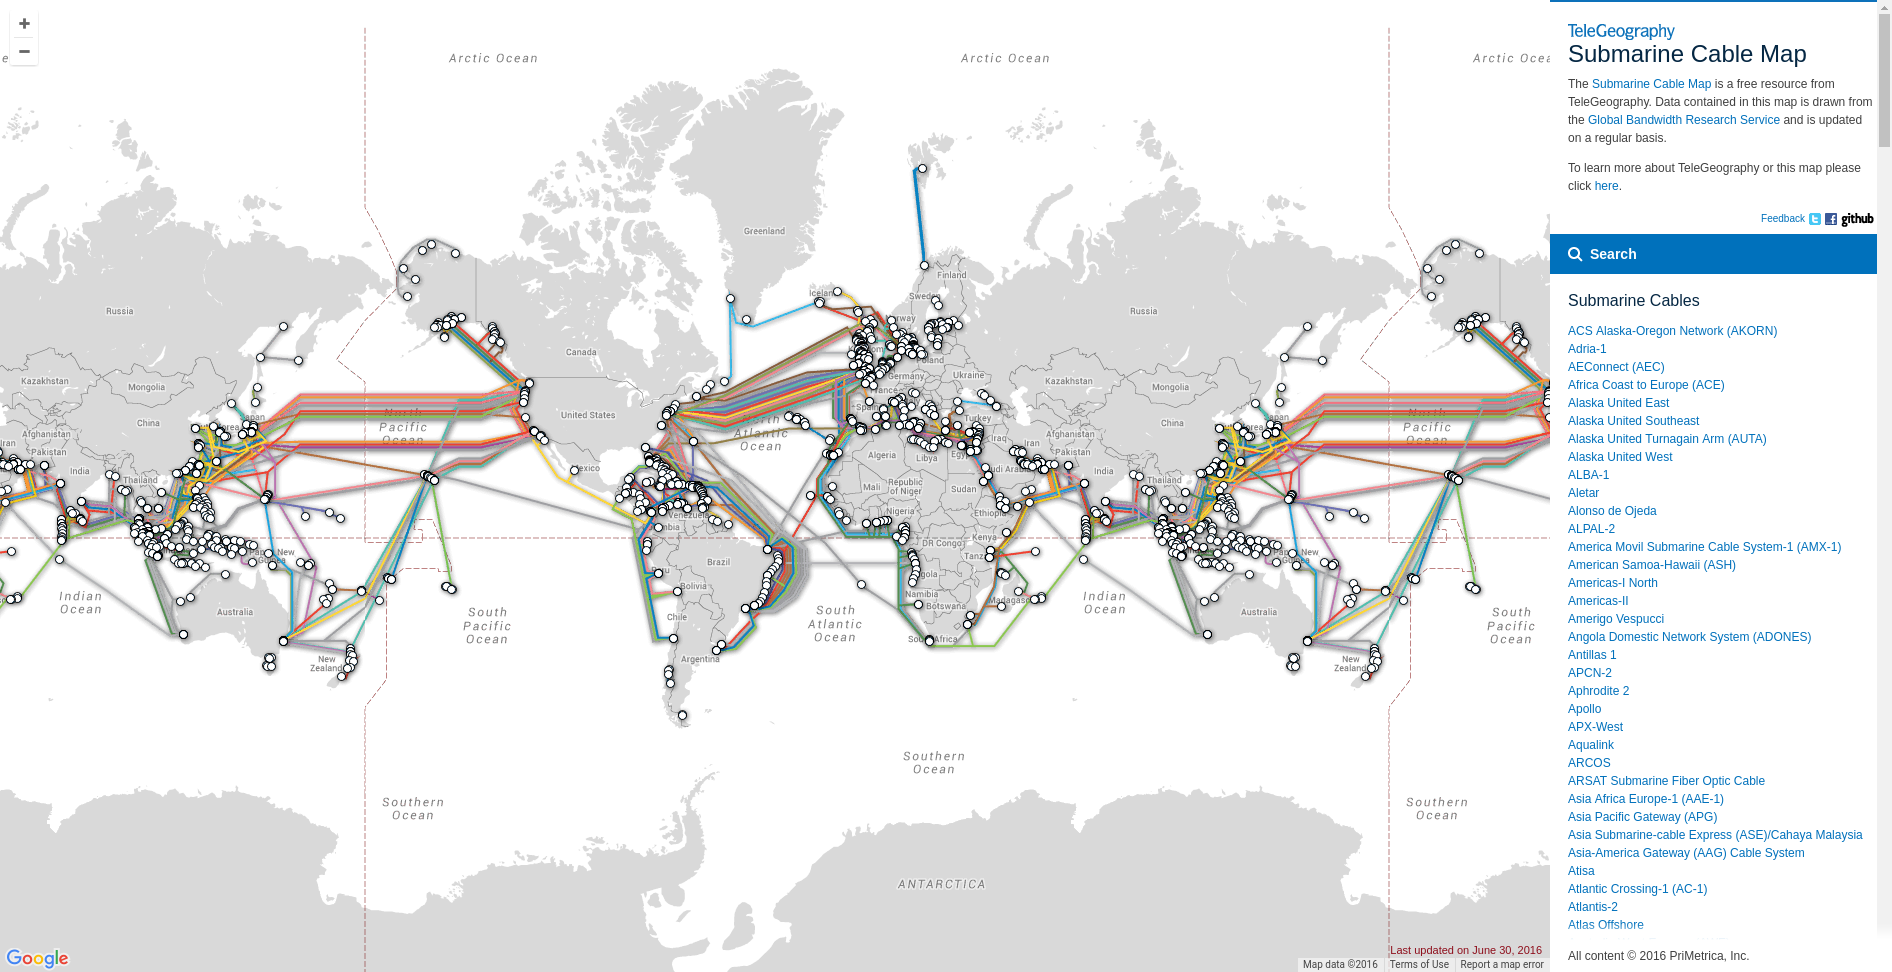
\includegraphics[width=0.8\textwidth,keepaspectratio]{images/geovis/submarine.png}
% \caption[
%     TeleGeography’s free interactive submarine cable map, Urldate: 07.2016 \newline
% \small\texttt{\url{http://www.submarinecablemap.com/}}
% ]{TeleGeography’s free interactive submarine cable map}
% \label{fig:submarine}
% \end{figure}

% \begin{figure}[h]
% \centering
% 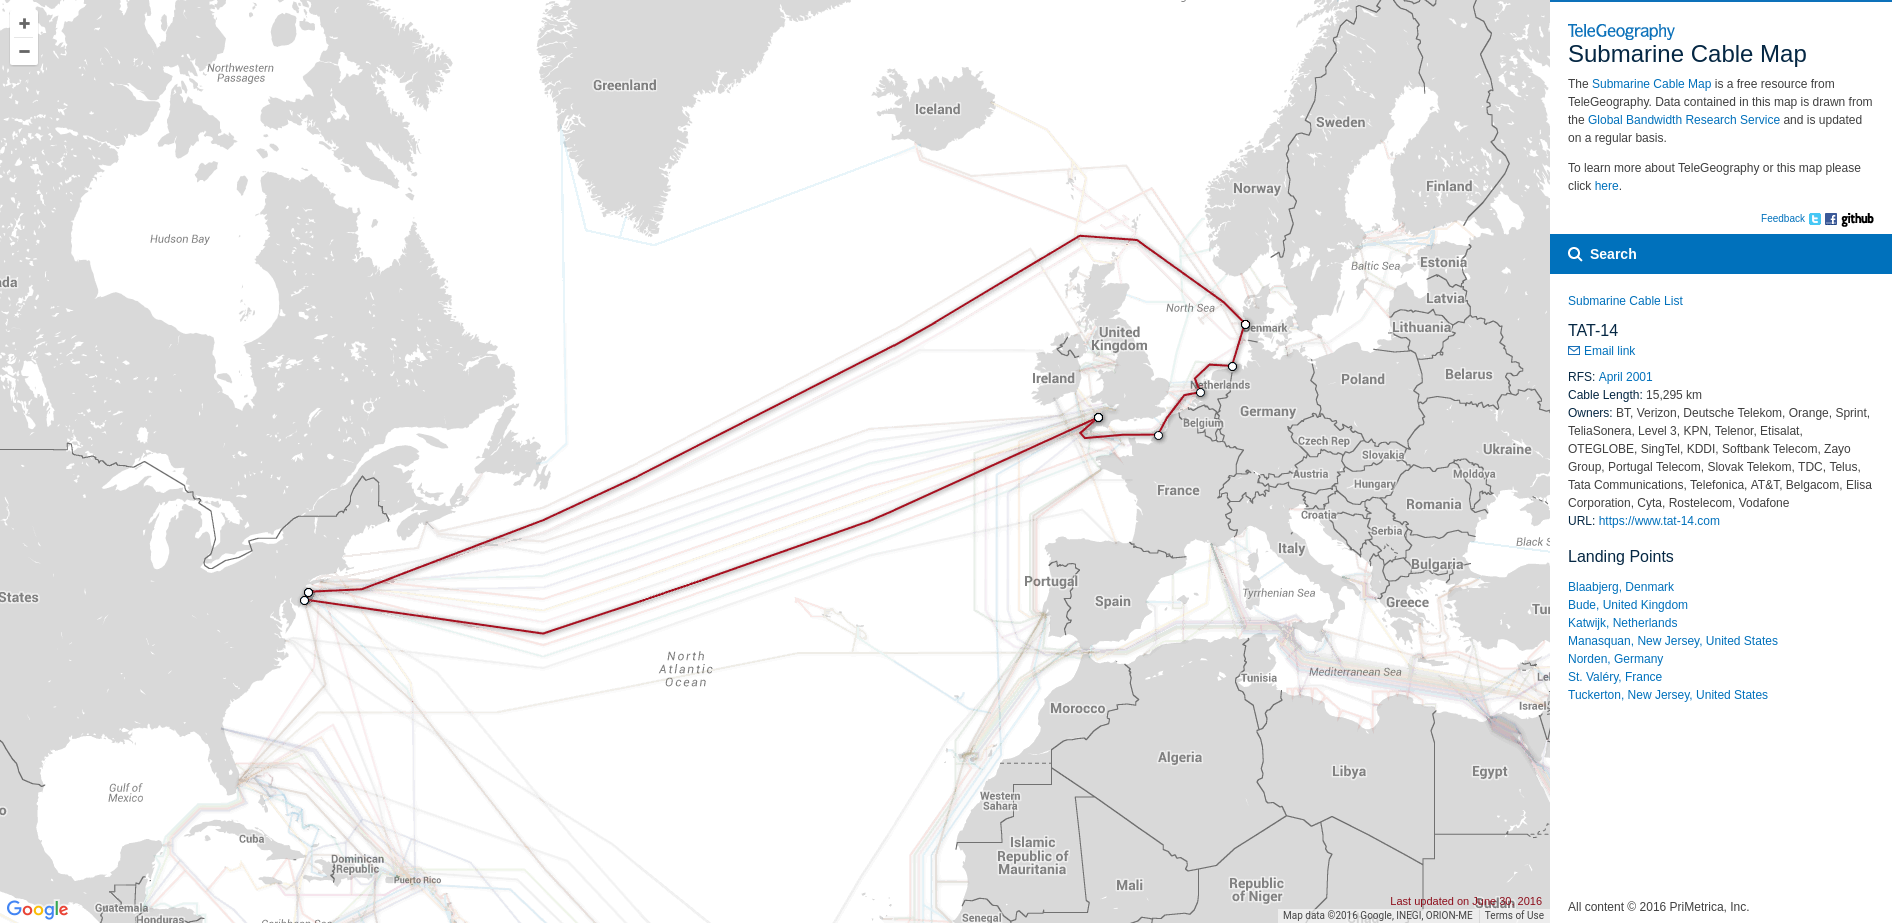
\includegraphics[width=0.8\textwidth,keepaspectratio]{images/geovis/submarine-interactive.png}
% \caption[
%     TeleGeography’s free interactive submarine cable map, Urldate: 07.2016 \newline
% \small\texttt{\url{http://www.submarinecablemap.com/}}
% ]{TeleGeography’s free interactive submarine cable map}
% \label{fig:submarine-interactive}
% \end{figure}

% \item[E-commerce] \hfill \\
% \ac{GeoVis} can be very useful in analysing data provided by e-commerce shops if they track online orders with some kind of geographical information. If such data is available and provided, it is possible to easily visualize the target group of a company on a map and therefore  create knowledge and allow for generating hypothesis i.e. the next region for expansion.

% \end{description}